\setchapterpreamble[u]{\margintoc} % Uncomment for a table of contents in the margin, NOTE: top 3 references overlap with this so this will need fixing if the margin toc is desired
\chapter{Introduction}~\label{chapter-introduction}

\epigraph{`Begin at the beginning,' the King said gravely, `and go on till you come to the end: then stop.'}{Alice in Wonderland, by Lewis Carroll}

\bigskip

\begin{kaobox}
The core argument of the introduction chapter can be summarised as:

\textbf{Context}
\begin{enumerate}
    \item Mobile apps are an important category of software
    \item Achieving quality in software is challenging
    \item Quality is particularly important for mobile app developers because of the way the ecosystem works
\end{enumerate}

\textbf{Motivation}
\begin{enumerate}[resume]
    \item Software analytics can help improve quality, particularly with respect to reliability by gathering and analysing data relating to failures during real-world use.
    \item Analytics can be especially important for improving mobile app reliability because there is a huge diversity in devices and contexts where mobile apps are used, which can affect reliability of the apps.
    \item However, we have limited understanding of how software developers apply mobile analytics in practice for improving app reliability.
\end{enumerate}

7. To address this gap, we study the use and utility of mobile analytics by multiple Android mobile app development projects, the largest and most ubiquitous mobile app ecosystem.\sidenote{By expanding this with some explanation of the case studies used to study the research gap, covers what needs to be discussed for the *Research Focus* }


This leads on to the RQ and explanation of the 6 perspectives, sub-questions, and contribution

\textbf{Note}: Points 3, 4, and 5 above will be used to focus what is presented in Chapter 2 and Chapter 3.
\end{kaobox}

% This should cover the problem the thesis addresses, the aims and questions, the thesis structure, a summary of the main findings and a discussion on the thesis' contribution. It should prime the reader for what's about to come by providing an overview of what lies ahead.

% Establish your research territory by situating your research in a broader context.
% Establish and justify your niche by describing why your research is needed.
% Explain the significance of your research by describing how you conducted your research.

Billions of people use mobile apps on two main mobile platforms, Google Android and Apple iOS, and their related operating systems.  Android is integrated into additional mobile platforms including Kindle OS and various \glspl{oem}, particularly Huawei with HarmonyOS. There are millions of these mobile apps developed by millions of developers across the globe. Failures in these apps can adversely affect the experiences of end-users~\sidecite{bbcnews2020_nhs_covid_19_app_bluescreen_glitch}, businesses who provide apps, and/or goods and services provided through mobile apps. Failures can even adversely affect peoples' lives, for instance in China when the Covid-19 tracking app crashed people were stuck at hospital entrances and other checkpoints unable to enter, and travel plans were in chaos~\sidecite{scmp2021_chinas_covid_19_tracking_app_crashes} and in India where users were not able to book vaccinations as the app crashed~\sidecite{moneycontrolnews2021_cowin_apps_crash}.

The research presented in this thesis explores how the quality of mobile app software can be improved through the use of data gathered from various mobile analytics tools. Before presenting the focus of this research in more detail, we some of the background context pertaining to this research and how analytics can play a role in helping developers improve quality.\sidenote{How can I improve the rest of this section, until the Research Focus section please? E.g. would reordering the paragraphs help?}

%\subsection{The essence of analytics}
Achieving quality in software is challenging: software is not perfect and no developer can create perfect software, not even the leaders in the field.

\newthought{Software is not perfect}: it is formed through numerous human endeavours using flawed tools and techniques.
Bugs are ubiquitous in software, and no practical software is bug-free. Even one of the most respected software engineers, Donald E. Knuth, recognises, publicly acknowledges, \emph{and pays for}, bugs found in his creations. % ~\sidecite{knuth_trutex, wikipedia__knuth_reward_checks_2020}. 
\emph{``You are entitled to a reward of at least 0x$1.00 \nobreak\hspace{.16667em plus .08333em} ($2.56) if you are the first person to report a \textit{bona-fide} error not on those lists."}~\sidecite{knuth_the_bank_of_san_serriffe}. And self-aware developers expect that there will be bugs in their software. Nonetheless those involved can improve software through their choices and practices.

\newthought{Nobody is perfect}: even leading technology companies release software that crashes some have the misfortune to release software that crashes many other apps inadvertently, as Google discovered in Spring 2021~\sidecite{bbcnews2021_google_fixes_crashing_android_app_issues}. App developers, including the BBC for their iPlayer app, posted advice to end users about the issue in Google Play~\sidecite{bbc_iplayer_app_april_2021_webview_information} as the adverse effects of the bugs introduced by Google were so widespread.

Quality is particularly important for mobile app developers because of the way the ecosystem works.

\newthought{Surviving as an app developer}: app developers need to deliver software that can be used successfully by end users. To do so they need to be able to create software, package it as an app, and distribute it so it is available to end users.
%
They need to do so in a timely manner - perfection may be too long to wait for! Therefore developers need to balance and make tradeoffs in the work they do and don't do. \emph{``Bad decisions cost money (and reputation) so we need better tools for making better decisions."}~\sidecite[][p.115]{tantithamthavorn2021_actionable_analytics_tell_me_what_to_do}. The article also observes developers also need to decide what to avoid doing. Therefore developers need help to decide which failures are appropriate to fix now (and which to leave be).

End users need to be able to install and use the app. If the app is sufficiently usable and useful and behaves adequately, they may continue to use it. Developers cannot assess \emph{a priori} whether their app will meet the needs and expectations of users, or the needs of their stakeholders.
% Briefly explain why they can't...
%  - Product/Market fit
%  - Marketability of apps~\sidecite{nayebi2017version}, via App Store Effects paper: ``Nayebi et al. subsequently investigated open-source app versions that are not shipped into the app store [46], introducing the concept of release ‘marketability’. To this end, they surveyed 22 developers, the majority of which (95 percent) state that market acceptability of a mobile app release is more important than that of traditional software."
%  - Competition in the app store
%  - They're not in control of their destiny, the app store and the customers decisions have a major impact
%  - Adopting of the app and use of the app
% - Survivorship in the app store ecosystems and what devs can do to increase their app's survival~\sidecite{lee2014_determinants_of_mobile_app_success_evidence_from_the_app_store_market} Seller [app developer]-level decisions, app-level decisions, user response to the decisions. It doesn't discuss app store algorithms or their effects. c.f. the more recent articles on iTunes rankings of apps from Medium.com
In short, they cannot predict whether their app will thrive.

\newthought{Crashes can leave indelible, adverse, results}. An increase in crashes led to an increase in `churn'~\sidenote{Churn is also known as attrition and is used to measure users who leave a collective group over a specific period~\href{https://en.wikipedia.org/wiki/Churn_rate}{en.wikipedia.org/wiki/Churn\_rate}.} of up to six times the average rate of churn according to industry reports~\sidecite{levy2016_crash_and_churn_report, levy2017_the_crash_and_burn_report_findings}~\sidenote{Note: Apteligent was acquired by VMWare in 2017 and few of their online materials remain available.}. 
Facebook deliberately tested the tolerance of users by introducing automatic crashes in their Android app, according to~\sidecite{efrati2016_facebooks_android_contingency_planning}, to measure when users would abandon the app entirely. %Found via https://9to5google.com/2016/01/04/facebook-intentionally-made-its-android-app-crash-to-test-how-addicted-users-are/ 

In terms of bugs mobile developers face,~\emph{``... automatic in-app crash reporting is the most prolific channel of reporting bugs..."}~\sidecite{alsubaihin2019app_store_effects_on_software_engineering} % Full sentence: While automatic in-app crash reporting is the most prolific channel of reporting bugs, the one mostly prioritised by our respondents is user reviews in app stores.
-- presumably as there are many crashes in mobile apps, otherwise it wouldn't be a prolific source. 

A survey in Germany reported that the most important annoyance for users was instability, ~\emph{i.e. ``instability (app crashes at startup or in certain cases) with 41\% of all responses"}~\sidecite{nitze2015_a_survey_on_mobile_users_sq_perceptions_and_expectations}.  %Then, users were asked (unsupported) for what they find annoying about using mobile apps. The most important aspect mentioned was instability (app crashes at startup or in certain cases) with 41% of all responses
%SHOULD-DO extend this paragraph with other references. For now I've merged it with the next paragraph.
%


\newthought{Stability}: is a prerequisite for an app to be viable in the marketplace, and several key app stores clearly state unreliable apps (~\emph{e.g.} apps that crash) will be marked down and possibly ejected from the app store~\sidecite{appleappstore2021_app_completeness, google_play_policy_center_broken_functionality, huaweidevelopers_appgallery_review_guidelines}. For example, Apple states~\emph{``On average, over 40\% of app rejections are for Guideline 2.1 – Performance: App Completeness."}~\sidecite{appleappstore2021_review_avoiding_common_app_rejections} with crashes and debugs listed as the first rejection reason. % Crashes are undesirable yet commonplace; therefore one of the key software qualities in use where analytics may be able to help measure and improve reliability for end users.
Crashes are undesirable yet commonplace; therefore they are a good candidate for evaluating how analytics may be able to a) help measure them and b) help developers to address them, in order to improve the reliability of mobile apps for end users.
% See also a developer's question about releasing iOS apps with known crashes https://developer.apple.com/forums/thread/68770

Conversely, Android apps that score highly in terms of stability may be selected to be promoted and featured in Google Play. One of the developer-oriented Google Play Guides provides an imperative: `Improve your app’s quality and discoverability'~\sidecite{android_store_listing_guide} which combines with the Google Play Guide on Android Vitals. This states: ~\emph{``Apps whose metrics are higher have greater promotability, which raises their ranking in Google Play Store searches. They also are more likely to be eligible for the New \& Updated and Editor's Choice collections on Google Play, and to be nominated in the Google Play Awards."}~\sidecite{android_android_vitals_guide}. % See also https://blog.embrace.io/top-5-reasons-your-app-is-losing-discoverability-on-google-play-store/

\medskip

Research motivation: Software analytics can help improve quality, particularly with respect to reliability by gathering and analysing data relating to failures during real-world use.

\newthought{Software Analytics}: exist and are used across and throughout software development practices, and they can be used to better understand and improve these practices and the resultant software~\sidecite{buse_analytics_2010, buse2012_information_needs_for_software_development_analytics, menzies2018_unreasonable_effectiveness_of_software_analytics}. A major source of software analytics is generated through use of the software, \emph{i.e.} use of mobile apps in the context of this research.

\begin{kaobox}[frametitle=Usage data]
%\newthought{Usage data}: 
Usage data
can be generated by actual users, emulated by other people, simulated by automated scripts interacting with apps, generated by programs, and fabricated by providers of mobile analytics tools/services. Of these, usage generated by actual users is inherently part of the real-world microcosm developers of the apps inhabit and therefore the research methods need to understand the use of mobile analytics in this context. 

There may be various ways to access the real world data, such as being a part of the development team, or being granted access by the development team. While the providers of the mobile analytics services may also have access various ethical, commercial, non-disclosure, safeguarding, and additional considerations make such access unlikely even though it could be tremendously rich and insightful. Some of the research can be performed using emulators and/or simulators and allows for greater control of the input conditions.
\end{kaobox}

Analytics can be especially important for improving mobile app reliability because there is a huge diversity in devices and contexts where mobile apps are used, which can affect reliability of the apps. However, we have limited understanding of how software developers apply mobile analytics in practice for improving app reliability. To address this gap, we study the use and utility of mobile analytics by multiple Android mobile app development projects, the largest and most ubiquitous mobile app ecosystem.


\newthought{The big picture}: broadly, this research aims to understand whether mobile analytics can help developers to improve the reliability of their apps. A second applied research area emerged as various flaws and limitations were discovered in the various mobile analytics tools and services, to discover and categorise the flaws and limitations, and to consider some of the effects on actually improving app quality given these flaws and limitations.

\newthought{Scope and delimitations of this research}:
% https://www.phdstudent.com/thesis-and-dissertation-survival/research-design/stating-the-obvious-writing-assumptions-limitations-and-delimitations/
of the various forms of mobile analytics this research concentrates on \textbf{platform-level analytics} together with \textbf{crash and error analytics}. It applies these forms of analytics with a focus on improving \textbf{stability} of Android apps available in the Google Play Store.

\newthought{Google Android chosen}: this research focuses on the most used operating system -- Android -- in its most popular and mature platform -- Google Android -- to discover whether mobile analytics can help developers improve the stability of their apps by fixing bugs that adversely affect their stability.

\newthought{Smartphone-like devices}:
the research focuses on apps that can be installed and run on smartphone-like devices, including tablet devices\sidenote{There are various forms of mobile device such as 3G battery powered routers which are outside the scope of this research.}.

\newthought{Ubiquitous Android Vitals}: a default mobile analytics service, called Android Vitals~\sidenote{Android Vitals is integrated into \myindex{Google Play Console} which provides additional functionality including app store metrics, ratings and reviews, release management, and so on.}, is integrated into the Google Android platform and available free of charge for all developers of apps in the Google Play app store. So, it was selected as the core analytics tool for this research, as it is prevalent, and also one of the quality signals Google uses to decide whether to promote apps in its app store. % Isabel suggests a diagram of the ecosystem would be useful around now.

\newthought{In-app crash reporting}: the research into this default mobile analytics service is complemented with research in additional analytics tools that include in-app crash reporting to provide perspective and contrast on their various characteristics and capabilities. %(How in-app crash reporting works is discussed in the appendix \href{{app:crash-recording-and-reporting-in-android}}{\nameref{app:crash-recording-and-reporting-in-android}}.) 
In app crash reporting is used in at least 80\% of Android apps in Google play according to AppBrain's\index{AppBrain} analysis of Crash Reporting libraries~\sidenote{\url{https://www.appbrain.com/stats/libraries/tag/crash-reporting/android-crash-reporting-libraries}}.

\newthought{No panacea}: in-app crash reporting is not a panacea. Not all apps use it for various reasons, and not all crashes are reported by in-app crash reporting. For instance, crashes that occur when the app starts, or while an app is still being initialised, may not be detected or reported. Additionally not all failures are crashes, for instance Google Android and Huawei AppGallery consider application freezes, known as ANRs, to be failures too. Therefore this research takes a holistic approach to managing failures that extends beyond the analysis of crashes reported using in-app crash reporting.   % SHOULD-DO forward-reference to a discussion on crashes at startup and comments made by the Google Play Console PM about these types of crashes.

%\akb{While it is right to focus on specific analytics, don't forget to explain the rationale for the ones you have chosen.} Agreed and will do when the content is migrated.

% \yijun{Should talk about quality (echoing the title), then talk about reliability and other quality issues.} \url{https://developer.android.com/docs/quality-guidelines/core-app-quality}~\sidecite{android_guidelines_core_app_quality}

\medskip
\newthought{Determining quality}: one of the key considerations for app developers is whether the quality of their apps is adequate. There are many ways developers can assess quality of apps, including static analysis, in-person testing, and automated testing. Users may perform their own subjective assessments of quality, and some of these users provide feedback in the form of ratings and reviews. Researchers have investigated these various sources of quality-related information (these will be discussed in Chapter 2). This research concentrates on using sources of analytics related to usage of apps to help developers a) assess the quality of their current software, and b) improve the quality using the same analytics sources.

% MUST-DO either here, or move this to the related works chapter:
% As Febrero, Moraga and Calero note:~\emph{``Software Quality is a multidimensional concept for which Reliability is considered as a key attribute."}~\sidecite[][p.224]{febrero2017_software_reliability_as_user_perception}. Over thirty years after \textbf{MUST-DO} expand on Muse's views...

\medskip
\newthought{Success/failure factors}: % TODO improve this heading
in the preceding paragraphs several factors have been identified that pertain to the success of mobile apps, namely the success, or failure, ...
\begin{enumerate}
    % \setlength\itemsep{-0.5em} %\itemsep0em
    \item to deliver perceived quality for the end user, measured by churn as a proxy, because users do not change software if they can help it. %SHOULD-DO investigate research into stickiness?
    \item for developers to be able to work productively on providing new features \emph{etc.}, rather than spending lots of time working on failures.
    \item of being able to use crash reporting as a trustworthy and effective source of information about failures of apps.
    \item for developers to triage and address failures that do occur efficaciously so they stop being a prolific source of bugs.
\end{enumerate}
% Therefore, one success factor for developers of mobile apps is in addressing crashes so they stop being a prolific source of bugs.

\newthought{Rationale}: 
the rationale for selecting Google Play Console with Android Vitals include the vast scale and reach of the platform-level analytics in the largest app store globally where potentially billions of users rely on the quality of these apps and millions of developers have to trust and rely decisions that the Google Play store ecosystem applies for the apps they release in the app store. Furthermore the majority of Android apps include at least one analytics library that collects and reports crash and error analytics. Both users and developers \emph{de-facto} trust these libraries are well behaved and can be depended on. Similarly users implicitly trust developers not to do net harm. 
% For more reading on the nuances of the actions of doctors see:
% https://www.bmj.com/content/366/bmj.l4734/rapid-responses which includes a detailed clarification of "In illnesses one should keep two things in mind, to be useful rather than cause no harm".
% The thesis discusses various aspects of \myindex{trust} shortly. %MUST-DO x-ref where I do.
% https://www.statista.com/statistics/736576/trust-mobile-apps-smartphone-users/ from 2017 survey data. 

Case studies were used to study the research gap as they provide real-world, \emph{in-situ}, microcosms of the use of mobile analytics for apps that have external user-bases (rather than research based on students, friends and family, and so on). 

\section{Research Focus}~\label{research-focus-section}
\vspace{-6mm}
\begin{quote}
    \emph{``...there are several companies that collect operational data from mobile apps that have been installed on millions of devices. Most of these companies provide the app developers with the data and some rudimentary analysis on them. There is a wide variety of reliability and performance problems that can be solved by building tools and approaches that mine such operational data...''}~\sidecite[][p. 28]{nagappan2016_future_trends_in_sw_eng_for_mobile_apps} 
\end{quote} 

This quote helps provide the context of this research into the use of mobile analytics to help app developers improve the reliability/stability of their mobile apps.
%
Research into the use and efficacy of software usage analytics appears to be under-served (this will be discussed in Chapter~\secref{chapter-related-work}), particularly in terms of being able to use the analytics to identify and potentially address quality flaws in apps in use.

The domain of mobile apps was selected for this research as mobile apps are ubiquitous, extremely popular, and have interesting and challenging contexts of use. Within this domain the research ended up focusing on Android apps for various reasons including: the analytics tools available, the relative glut of suitable apps available for research, my prior experience and expertise, and their market share. Furthermore, in recent years, platform-wide analytics have been made available to all the developers of actively-used Android apps in Google Play. Despite the ubiquity of these platform-level analytics, there appeared to be no research into their efficacy, completeness, or accuracy.

%\subsection{On Android}
From a research perspective focusing on the \textbf{Android} platform is also credible in terms of specialising the research focus given its mainly opensource codebase and popularity as a platform (Number 1 globally). Android is also well researched, for example with 
\href{https://conf.researchr.org/search/icse-2022/android/events}{40} papers on Android (of these 3 also included iOS) % 53 papers on the topic at ICSE 2020 and related conferences and workshops 
, whereas only \href{https://conf.researchr.org/search/icse-2022/ios/events}{2} % 3 in 2020
papers were exclusively focused on the extremely popular iOS platform at the preeminent \gls{icse} \href{https://conf.researchr.org/home/icse-2022}{2022} conference and related workshops. Android, therefore, has much richer range of prior-art to build on; and any improvements in mobile apps via this research has the potential to effect improvements in the largest of the mobile ecosystems.
% ICSE iOS  papers:
% https://doi.org/10.1145/3524613.3527803
% https://doi.org/10.1145/3524613.3527813

The research also touches on \textbf{software testing} mainly in terms of prior art and in practices of the development teams. Automated tests were developed during the Commercial, \myindex{C1}, app-centric case study to reproduce a major crash that caused a spike in the crash rate and they measured the improvement in the crash rate using mobile analytics when the underlying fix was released. Mobile Analytics complemented automated tests and interactive testing by providing objective measurements of the stability of the apps. The research did not encompass many improvements in software testing practices, nonetheless it identified that Google uses usage analytics to determine which locales to use in their automated `robo'\index{Robo} testing as part of providing pre-launch reports.

\begin{figure*}
    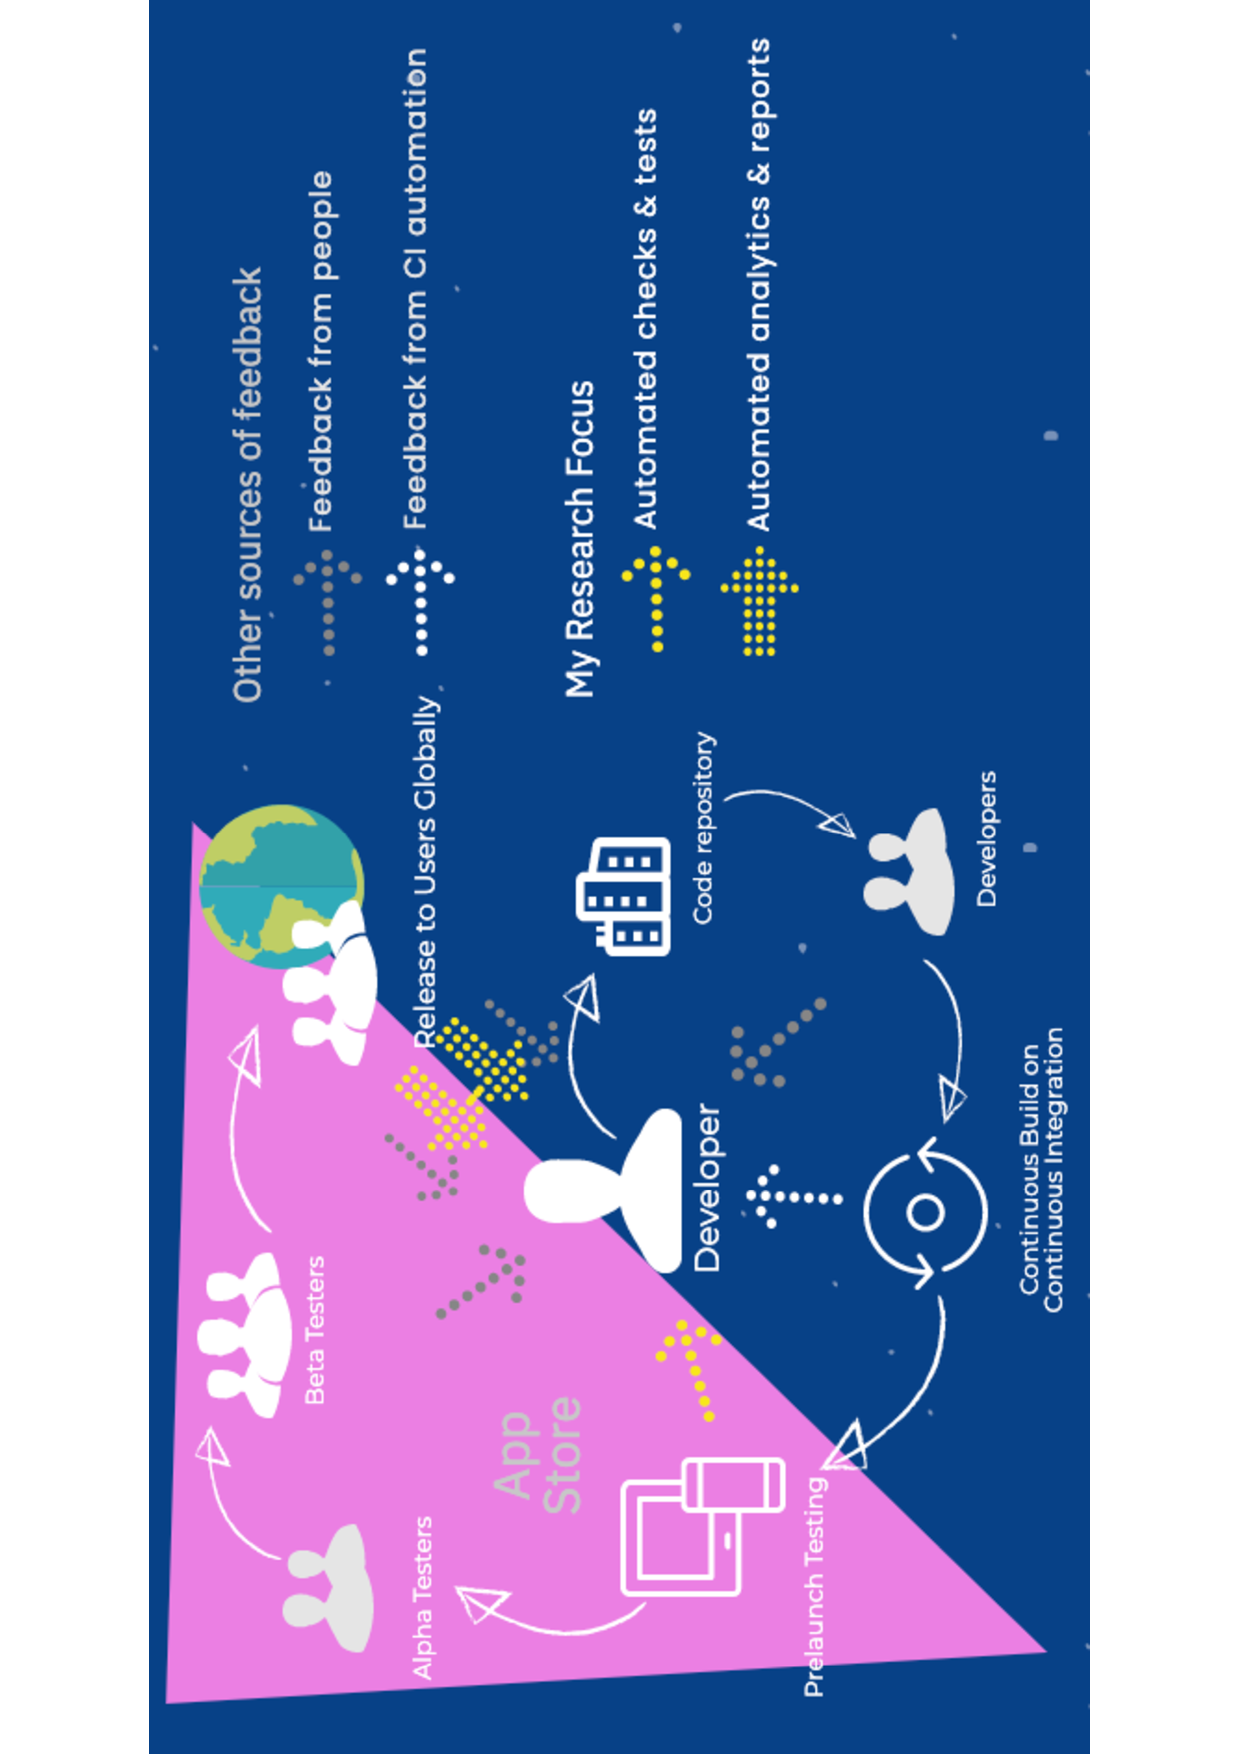
\includegraphics[width=\linewidth]{images/mobilesoft/silvias-developer-centric-figure-mobilesoft2020.pdf}
    \caption[Sources of feedback for developers]{Sources of feedback for developers \\The Research focuses on automated checks and tests performed by the app store, automated analytics and reports both in-app and at the platform level. \\ \\Other sources of feedback available to developers includes feedback from people and feedback from their development tools and CI automation.}
    \label{fig:sources-of-feedback-for-developers}
\end{figure*}
% Source \url{https://create.piktochart.com/teams/16497973/infographic/saved/47760961?}

% TODO if the following footnote is split across 2 pages then review https://texfaq.org/FAQ-splitfoot to prevent an entire page becoming a hotlink for the URL in the footnote.
Developers have various sources of feedback about their apps, as Figure~\ref{fig:sources-of-feedback-for-developers} illustrates~\sidenote{The image was created in pikochart, a paid for online editing tool. Thanks to Silvia Harty for her help designing the original figure.}. The pink triangle represents the extent of Google Play (the app store) in terms of providing feedback. Other feedback is also available independently of the app store, for instance: from the development process, and by using software incorporated directly into the app that provides bi-directional communications between the development team and end users~\sidecite{avellis_harty_yu_towards_mobile_twin_peaks}.


Each source of feedback may stem from humans (for example, in reviews) or from software (for example, from code quality tools such as Lint).This research introduces three sources of software-generated feedback:
\begin{enumerate}
    %\setlength\itemsep{-0.5em} %\itemsep0em 
    \item prelaunch testing\index{Prelaunch testing}: automated checks and testing provided by the app store (Google Play) as part of their \gls{plr},
    \item platform-provided analytics\index{Platform-provided analytics}: automated analytics and reports gathered by the Google Android platform from users devices configured to provide the underlying data,
    \item in-app error reporting (including crash reporting): software added by the app development team to detect and report crashes, and optionally errors and similar/related data.
\end{enumerate}

% NB: Alpha and Beta channels formed part of one of the major industry case studies. Clearance has not yet been granted to write or publish the findings.

Note: while the first two of these sources use Google Play as their source, other app stores and similar ecosystems may provide equivalent sources of feedback.

\section{Research Questions}
\label{section-research-questions}
%%%%%%%%%% Isabel Evans suggests adding a table with my RQs at the start of this section. TBD. COULD-DO. Certainly it seems this section needs polish.

%MUST-DO \yijun{If possible, you may need to dig out a few MobileSoft research papers to give evidence that these research questions have not been addressed in literature, e.g., \emph{Future Trends in Software Engineering Research for Mobile Apps}~\sidecite{nagappan2016_future_trends_in_sw_eng_for_mobile_apps}, whether the future work of some paper suggests one does not know the sources, value, or impact of mobile analytics to assess and improve app quality? Is there nothing in the general SE literature studying the "analytics" to "general software quality" problem? If there are such general work, how does "mobile analytics" and "app quality" differentiate the RQs to existing ones...}


My research hypothesis is that using mobile analytics can help improve the work development of teams and the quality of the products they create. Here work includes the development, testing, and bug investigation of the software being created. For the quality of the product, this research is focusing on a subset of qualities which are \gls{glossary-technology-facing}, %technology-centric, 
and in particular the \gls{glossary-reliability} and \gls{glossary-stability} of the mobile apps when they are in use. This research builds on prior work on software analytics for mobile apps and focuses on its practical application by software development teams to improve app reliability. This is important because app reliability, as measured by crash rates and ANRs, is key metric in the mobile app ecosystem. Because this metric is used by the platform provider to determine whether an app should be given access to the ecosystem, it is something developers should pay attention to. In order to understand the effect of applying mobile analytics on the software development practices for improving reliability of apps, we need to explore the processes, artefacts and tools associated with these activities. This research investigates these three dimensions based on case studies of different mobile app projects, to identify both the current practices and opportunities for improvement provided by using mobile analytics.

The core question investigated by this research:

\begin{quote}
  \emph{How can applying mobile analytics in software development practice improve the reliability of mobile apps?}~\label{overall-research-question}\index{Research questions}
\end{quote}
% Thanks to https://tex.stackexchange.com/questions/35933/indenting-a-whole-paragraph

To expand on the research question:
\begin{itemize}
    \item \textbf{Applying mobile analytics}: is the use of mobile analytics in order to effect improvements to the practices and the artefacts. Applying mobile analytics refers to both collecting data from the usage of the app and also making use of the analysis of this data to identify and address issues that can improve the app. Improvement of the app focuses on increasing the stability/reliability by reducing ANRs, crashes, and through improving how the app handles various errors (typically reported through Exceptions~\footnote{Exceptions are a core construct in Java programs intended to make those programs robust~\cite{robillard2000_designing_robust_java_programs_with_exceptions}, and similarly \glspl{glossary-exception} are core to Android apps}).
    \item \textbf{Mobile analytics}: Analytics where the data is collected by software running on mobile smartphone-based devices pertaining to the app's qualities-in-use. This research focused on analytics collected pertaining to the stability of the app, where stability includes the reliability of the app.
    \item Software development: includes tasks performed by the software developers including design, coding, testing, bug reporting, and bug tracking.  Use of Scrum development practices, following recommendations and guides that include application compatibility, \gls{ui} guidelines, and designing for performance and responsiveness, \emph{etc}. [Software] testing~\sidecite[][pp.398 - 399]{wasserman2010_software_engineering_issues_for_mobile_app_devt}.~\sidenote{This short paper skims over topics without evidence developers actually do them. Their survey, cited in this paper isn't available so appears to have not actually been published.}
    \item Reliability and Stability are two intertwined measures of software quality in use. There are contradictory opinions on their relationships to each other and to their contributions to software quality, these will be discussed in Chapter~\secref{chapter-related-work}. 
    \item In practice: the key scope of measurement focuses on the efficacy in real-world projects from the perspective of software practitioners who develop mobile applications.
\end{itemize}

In order to answer this research question it is appropriate to consider improvements to the \emph{app i.e. the product} and to the \emph{processes/practices} development teams apply when they develop and maintain their mobile apps. Improvements cannot be be usefully considered in isolation, they need to be grounded in the current practices: the developers will have their perspectives on their use of mobile analytics, and their development artefacts may provide cross-verification of what they say they do compared with tangible evidence of how they use those mobile analytics tools. 

Furthermore, there may be constraints and/or limitations in the current mobile analytics tools which may adversely affect the improvements development teams are able to make to their processes/practices and to their products, hence it is also germane to consider improvements to the current mobile analytics tools.

These additional supporting questions can be restated as six distinct yet related perspectives.

\begin{figure*}
    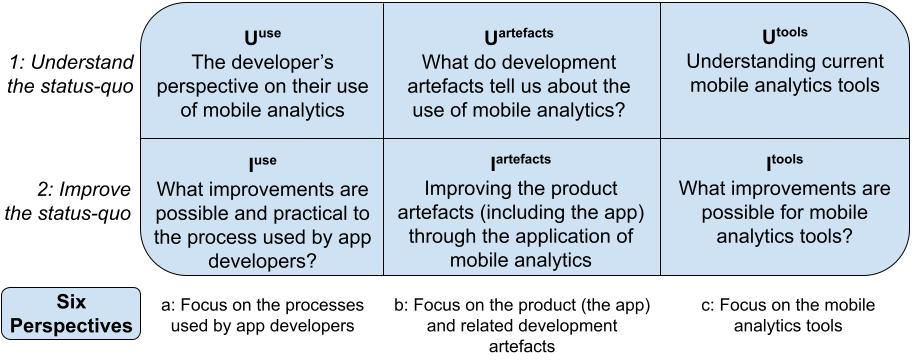
\includegraphics[width=\linewidth]{images/my/six-perspectives-2x3-matrix-12-nov-2021.jpeg}
    \caption{Six Perspectives of Mobile Analytics}
    \label{fig:six-perspectives-in-the-research-questions-section}
\end{figure*}

\subsection{Research questions lead to six perspectives}~\label{rq-leads-to-six-perspectives}
The six perspectives are illustrated in Figure~\ref{fig:six-perspectives-in-the-research-questions-section}~\sidenote{Source figure:~\href{https://docs.google.com/drawings/d/1SafKu3uqgl-s8-I8iWSSWmFY4NdlNpw8v6ZiJDGh50c/edit?usp=sharing}{Google Docs: Six Perspectives drawing}.} and paraphrased below:

\begin{enumerate}
    %\setlength\itemsep{-0.5em} %\itemsep0em
    \item [1a] What do app developers say they do in terms of using mobile analytics? (understand the \emph{status quo} from their perspective).\index{Research questions}
    \item [2a] What's possible in terms of improving their processes, their practices through using mobile analytics?)
    \item [1b] What does their source code (and other available development artefacts) tell us about their use of mobile analytics? (\emph{i.e.} to understand current behaviours in terms of the code that's implemented.
    \item [2b] What's possible in terms of improving the product (and particularly the mobile app) through the application/use of mobile analytics?
    \item [1c] What do we learn about various current mobile analytics tools?
    \item [2c] What improvements are possible for mobile analytics tools based on what was learned in the various case studies?
\end{enumerate}

These provide clear grouping for each of the three columns: on processes (a), on apps and related development artefacts (b), and on the analytics tools (c) which are considered in terms of first understanding and then improving the \emph{status-quo}, shown as two rows, \emph{i.e.} a 3x2 matrix. 


% https://www.skmurphy.com/blog/2014/01/27/difference-between-a-hypothesis-and-an-assumption/
Here the hypothesis is that analytics can help, as stated by Buse and Zimmermann ~(\citeyear{buse_analytics_2010}); and \emph{``with explicit and implicit feedback now available (almost) continuously, questions arise. How can practitioners use this information and integrate it into their development processes [to decide when to release updates]?"}~\sidecite{maalej2016_towards_data_driven_requirements_engineering}.


\section{Research contributions}
Before this research little was known about developers integrating mobile analytics into their artefacts and/or their processes. Unknown were - how, why, and when, they used the outputs of the mobile analytics. Similarly, the effects of using mobile analytics in terms of any changes to the reliability of these apps was not known. Furthermore, little was known about the mobile analytics tools and services used by app developers in industry or in real-world mobile apps.

\subsection{My contributions to knowledge}
The research contributes to the understanding of tools and information seldom available to research - of professional app developers, their artefacts, and of professional mobile analytics tools and services. 

\newthought{Processes}: 
My research contributes knowledge on the approaches various app development teams apply when they use mobile analytics including the selection, integration of code and services, and their application of mobile analytics to detect, identify, and address errors and failures reported by mobile analytics. It builds on prior research, for example, on Insight, and confirms their findings. It contributes new knowledge in the adoption platform-level and commercial in-app mobile analytics, including a) usage patterns by development teams ranging from individual  developers, small teams and large,  \gls{glossary-sharded}\sidenote{\href{https://en.wikipedia.org/wiki/Shard\_(database\_architecture)}{Wikipedia: Shard (database architecture)}} teams, and b) public opensource projects, hybrid projects that combined private and proprietary practices, through to a development team at a major corporation.

Some of the findings were surprising in terms of the patterns of use and in the efficacy of using mobile analytics to achieve significant improvements.

Development teams who embedded mobile analytics into their ongoing, core practices, were able to achieve highly reliable and stable apps. 

\newthought{Artefacts}: 
The research extended prior art in studies of opensource mobile app codebases, with a focus on the use of the most popular product offering: Firebase Analytics. Developers often incorporated multiple mobile analytics libraries into a single mobile app, each for a specific purpose. When developers addressed failures reported by mobile analytics they often modified the source code of the app; these modifications were generally small, yet the effects on improving the reliability/stability of the app were material. 

It also contributes insights from proprietary, commercial codebases and issue tracking artefacts where development teams intermittently filed bug reports for issues reported by mobile analytics.

\newthought{Mobile  Analytics Tools}:
The research identified characteristics of a wide range of mobile analytics tools that serve Android app developers in particular. It also found and  presents a range of flaws found in professionally-developed mobile analytics tools, including several of the most-used mobile analytics offerings.

The research contributes material relevant to professional app developers and to the developers of mobile analytics. 

Improvements were identified in all three areas and some of these were implemented during the research. 

Note: In addition to specifying my research contributions add explicit summaries of my contributions that have already been published.

\subsection{Practical impact of my work}
Several of the tool development organisations including Amplitude, Google, and Iteratively actively sought insights and updates from my research. They improved various aspects of their respective mobile analytics offering.

App developers who applied the techniques described in my research were consistently able to significantly improve the reliability/stability of their apps.


\section{Outline of this thesis}
At a high-level thesis is in three main parts: the preamble which includes chapters 1 to 5, the findings in chapters 6 to 8, followed by the discussion, conclusion, and future work in chapters 9 and 10. There are two short appendices: on thematic analysis, and additional details for some of the mini-experiments.

\bigskip

This thesis starts with an introduction to the context of investigation - mobile app development - together with an exploration of the state of the art. Based on this, the method adopted for conducting the research is presented before outlining the different mobile app and analytics tool case studies. Following this, the findings are set out, covering three thematic areas relevant to the use of mobile analytics: app development processes and the use of analytics, apps and their artefacts, and mobile analytics tools. Finally there is discussion of the findings together with potential areas for future work. A more detailed outline of the remaining chapters of the thesis is set out below.
% TODO revise the following before submitting the revised thesis.

\newthought{Chapter 2 | Preparing the ground}: this chapter prepares the ground for the rest of this thesis by explaining contemporary development practices for mobile apps. It then presents five conceptual models related to mobile apps. These are followed by several, relevant, practical details.

\newthought{Chapter 3 | Related work}: explores the state of the art relevant to software quality, software analytics, and the mobile app ecosystem.

\newthought{Chapter 4 | Methodology}: sets out the research approach adopted to gather and analyse data for the different case studies explored as part of the research.

\newthought{Chapter 5 | Overview of the case studies}: introduces each of the app-centric and tool-centric case studies using a consistent structure to make them easy to comprehend and to facilitate comparison.

\newthought{Chapter 6 | Findings - Analytics in use}: presents the key findings from the case studies relevant to the use of analytics by mobile app development teams.

\newthought{Chapter 7 | Findings - Apps and their artefacts}: discusses the findings relating to the software developed in the different mobile app case studies, together with their associated artefacts.

\newthought{Chapter 8 | Findings - Mobile analytics tools and their artefacts}: focuses on the mobile analytics tools explored during the course of the research and the different artefacts produced by these tools.

\newthought{Chapter 9 | Discussion}: explores the findings across the different perspectives of the research in relation to the wider literature of software quality and mobile app development practices.

\newthought{Chapter 10 | Conclusions and future work}: summarises the key contributions of the research and discusses avenues for further investigation.
